\section{Measures of Cognitive Distance}

In this section, we will introduce various measures.  We use the square root of a measure called the Jensen Shannon Divergence as our measure of cognitive distance (CD). The performance score is then

\begin{equation}
S = 1 - CD.
\end{equation}

In order to understand the usefulness and reason behind this measure this section introduces some preliminary measures which the Jensen-Shannon Divergence builds on and then formally defines our measure of cognitive distance.    
  
\subsection{The Shannon Entropy}

An important measure of ignorance is the Shannon Entropy, which is maximized whenever all possible events are believed to occur with equal probability:

$H(X)=-\sum_ip_i(x_i)\log(p_i(x_i)).$

The entropy of a stochasic process, $\{X_i\}$ is defined by 

$H(\chi)=\lim_{n\rightarrow\inf}\frac{1}{n}H(X_1, \ldots, X_n),$

when the limit exists, which in this case it does as it was picked by us. 
We can calculate, then, that the Shannon Entropy of the simple ``treatment'' system is $2.7$ and that of the complex one is $3.26$. However, distributions over larger alphabets tend to have higher entropy and for our purposes the entropy should be considered a relative measure over distributions of the same cardinality. 

Specifically, the maximum entropy for categorical variables with $N$ categories is $\log_2(N)$, which happens when for each category, $x_i$, its probability is $p_i(x_i)=\frac{1}{N}$. 

This fact can be appreciated on hand of a mental or computational experiment \citep{Cover13} where there is an automatic type writer that randomly prints a sequence of letters from an alphabet with $m$ members, where at each time, $t$, each member of the alphabet has an equal chance of $\frac{1}{m}$ to be chosen as the next member of the sequence. The type writer can produce $m^t$ possible sequences of length $t$, each of them as likely as any other. We then have that 

$H(X_1, \ldots, X_t)=\log(m^n)$ and the entropy rate is $H(\chi)=\log m$ bits per symbol. 

In the current case, we can substitute $m$ with the number of possible combinations (joint states) that $k$ binary variables can assume: $2^k$.
The simple system has $k=3$ binary variables and its maximum entropy (random type writer) belief has entropy $\log_2(N)=\log_2(2^k) = 3$. The more complex treatment system has $k=4$ binary variables and thus its maximum entropy belief has entropy $\log_2(N) = 4$. Entropy is also always positive, so that the measure is bounded between $0$ and the logarithm of the number of joint states $2^k$ that define the system. The Shannon Entropy is measured in bits when the base $2$ logarithm is used and it can be interpreted as the average number of yes or no questions a person needs to ask someone who knows the current outcome in order to gain knowledge of it.  In the worst case, this requires as many yes or no (high, or low) questions as there are binary variables, $k$. 

\begin{figure}
\noindent\makebox[\textwidth]{%      
        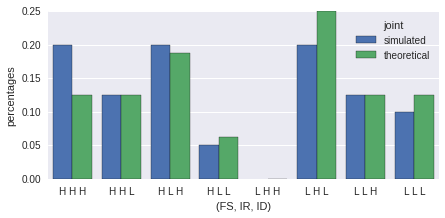
\includegraphics[width=1\textwidth]{figures/simplejoint.png}}
\caption{The limiting distribution of the simple treatment and an example frequency distribution pertaining to 400 random realizations.}
\label{fig:simplejoint} 
\end{figure}

But it is easy to see from a picture of the joint distribution describing joint behavior of the simple system (Figure \ref{fig:simplejoint}), for example, that very often three questions won't be needed. We could ask the person who knows whether the first variable, labeled ``Financial Sector'', has taken on the value ``H''.  If the answer is no, we could ask if the outcome is the event ``L'', ``H'', ``L'' and very often we would be right, finding the answer with only $2$ yes or no questions. Better yet, if we knew or somehow guessed the correct causal structure, we would know that whenever the ``Financial Sector'' variable takes on the value ``L'' and the ``Interest Rate'' variable assumes the value ``H'', the ``Industry'' variable must be in the low state. So, if we asked first ``is the value of the Financial Sector high'' and received ``no'' as an answer and then we asked ``is the value of the Interest Rate high'' and we received ``yes'' as an answer, we could be certain that the outcome must be ``LHL''. On average, for the simple system we would need to ask $2.7$ yes or no questions, if we know the distribution.   

\subsection{The Kullback-Leibler divergence}

The Kullback-Leiber Divergence was proposed as a measure of difference between two probability distributions $P$ and $Q$. Specifically, it was meant as a measure of the information that is lost when belief $Q$ is used as an approximation for a true probability distribution $P$:
\\

$D_{KL}(P(X) | | Q(X))=\sum_ip_i\log_2(\frac{p_i}{q_i}).$
\\

It is readily apparent that the Kullback-Leibler divergence can be re-expressed as follows:
\\

$D_{KL}(P(X) | | Q(X))=\sum_i (p_i\log_2p_i -p_i\log_2q_i = H(P, Q)-H(P)$, 
\\

where $H(P, Q)$ is known as the cross-entropy of $P$ and $Q$, and $H(P)$ is simply the entropy of $P$.

There are two problems with the Kullback-Leibler divergence as a measure of distance: 1) it is not symmetric ($D_{KL}(P | | Q) \not= D_{KL}(Q | | P)$) and 2) for the two distributions $P$ and $Q$, if one of the $q_i$ is equal to $0$, but the corresponding $p_i$ is not equal to $0$, the measure is not defined.  For example, we can see that when we simulated the complex process, some of the theoretically rare but possible outcomes have not yet occurred during the simulation and thus, if we want to measure the distance between the theoretical distribution and the frequencies of the simulated outcomes, using the Kullback-Leibler divergence, we will find that this measure is not defined. 

\subsection{The Jensen–Shannon divergence}

The Jensen–Shannon divergence is a symmetrized version of the Kullback-Leibler divergence that also solves the zero division problem:
\\

$D_{JS}(P | | Q)=\lambda*D_{KL}(P | | M) + (1-\lambda)*D_{KL}(Q | |M),$ 
\\

where $M=\lambda P + (1-\lambda) Q$ and $\lambda$ is usually, but not necessarily equal to $\frac{1}{2}$. In order for the measure to be symmetric, $\lambda$ has to be equal to $\frac{1}{2}$. 


The value of the Jensen-Shannon divergence is always between $0$ and $1$; $0$, when the two distributions are the same and $1$ when the two distributions have orthogonal support. This measure quantifies the amount of information in bits, about which of the two distributions one bit of data was drawn from, given that it was drawn from the first distribution with probability $\lambda$ and from the second with probability $1-\lambda$. For example, if the two distributions are the same, any bit of data will render no information about which of the two identical distributions it was drawn from, while if the two distributions have orthogonal support, each bit of data gives exactly one bit of information. To state this in Bayesian terms: if the two distributions are the same, then we can not learn from data and our posterior probability about which of the two distribution that data was drawn from is equal to our prior ($\lambda$ for the first distribution). At the other extreme, if the distributions have orthogonal support, the posterior will put probability $1$ on the distribution that supports the data; one bit of data carries one bit of information. 

\subsection{Cognitive Distance and the Performance Score}

If the square-root of the Jensen-Shannon divergence is taken, the result is a metric known as the Jensen-Shannon distance. This is the distance metric we use to calculate distances between any two distributions.  We refer to it as Cognitive Distance (CD):

\begin{equation}
CD(P, Q) = \sqrt{D_{JS}(P | | Q)}
\end{equation}

and to remind the reader, our performance score of person $i$ at time $t$, (supressing the index $i$), $S_t$, is 

\begin{equation}
S_t = 1 - CD(M_t, T),
\end{equation}

where $M_t$ is some person's Bayes Net model, at time $t$, of the true stochastic system, $T$. 
